\documentclass[tikz,border=10pt]{standalone}
\usepackage{tikz}
\usetikzlibrary{positioning}
\usetikzlibrary {arrows.meta}
\usepackage{tikz-feynman}
\begin{document}

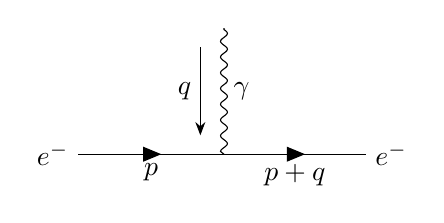
\begin{tikzpicture}
    \begin{feynman}
        %% fig j
        \vertex (j1) at (0,0);
        \vertex[right = -2.5cm  of j1] (j2){\(e^{-}\)};
        \vertex[right = 1.8cm  of j1] (j3){\(e^{-}\)};
        \vertex[above right = 1.6 cm and 0cm  of j1] (j4);
        % 对各个顶点连线
        \diagram*{
        (j2) --[fermion,edge label'=\(p\),] (j1)--[fermion,edge label'=\(p+q\)](j3),
        %介子连线
        (j4)--[photon, edge label=\(\gamma\), momentum'=\(q\)](j1),
        };
    \end{feynman}
\end{tikzpicture}

% \feynmandiagram [tree layout,horizontal=i1 to i2] {
% i1 [particle=\(e^{-}\)] -- [fermion] a -- [fermion] i2 [particle=\(e^{-}\)],
% b -- [photon, edge label=\(\gamma\), momentum'=\(k\)] a,
% };


\end{document}
